
% ------------------------------------------------------------------------------
% NUEVA SECCIÓN
% ------------------------------------------------------------------------------
\section{Funciona: Mempool completo}

%---------------------------Eden network---------------------------
\subsection{Eden network}

\textbf{Link:} \url{https://edennetwork.io/}

\textbf{Red disponible:} ETH

\medskip

Por el momento, esta el alpha por lo tanto las cosas pueden cambiar, estoy solicitando permiso para entrar medisnte websocket en discord y hasta ahora todavía no he tenido acceso, sin embargo el link \url{https://mempool.edennetwork.io/} puedes conectarte sin usar websocket (cosa que obvio no podemos usar)

\begin{figure}
    \centering
    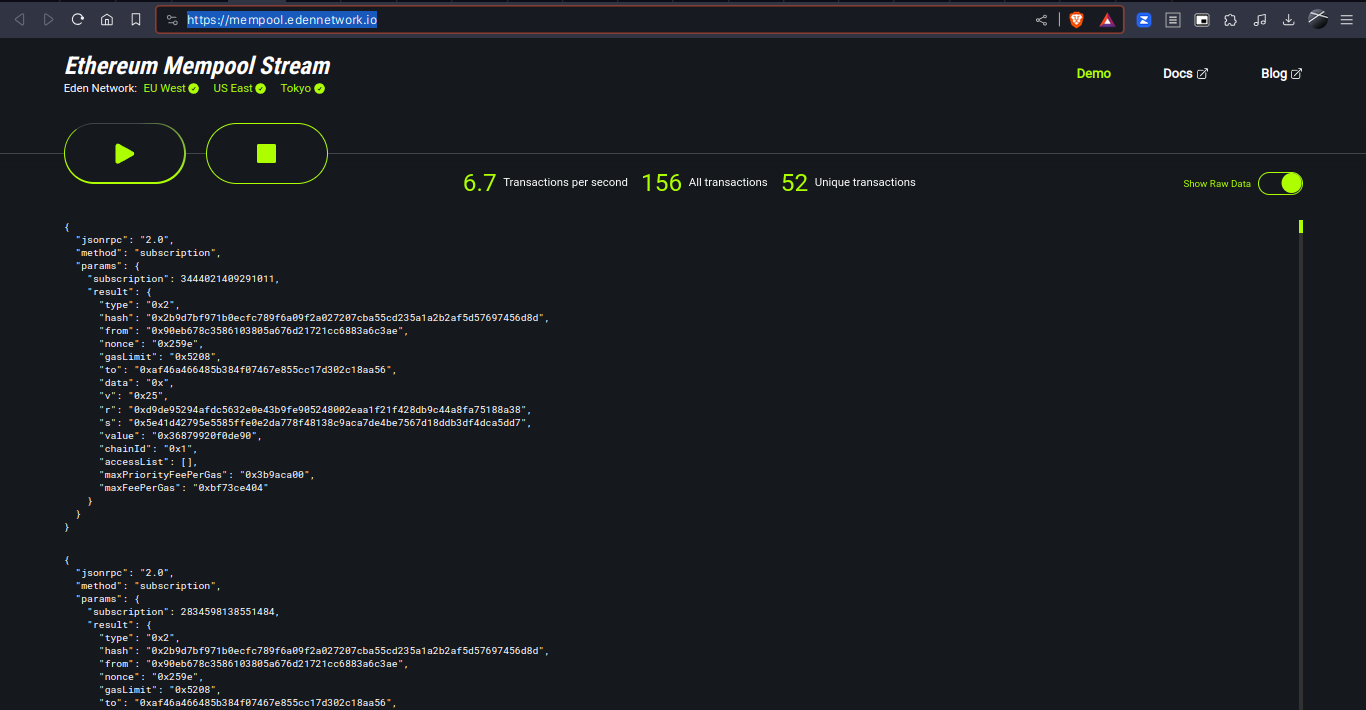
\includegraphics[width=1\linewidth]{img//screenshots/Screenshot from 2023-12-15 22-38-01.png}
\end{figure}

Se pregunto en el discord oficial acerca del uso de web sockets lo cual tras un par de horas se tuvo respuesta

\begin{figure}
    \centering
    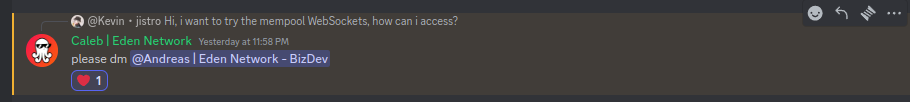
\includegraphics[width=1\linewidth]{Screenshot from 2023-12-16 00-09-47.png}
\end{figure}

Contacto: \url{https://discord.com/channels/761540124940697600/1152139988071350292/1185438359062061076} 

Al contactar con el desarrollador, este nos dio acceso al websocket el cual permite escuchar todas las transacciones en mempool pero sin la posibilidad de filtrado, aun así el desarrollador dijo que hay cosas sin documentar y es posible preguntar si hay la existencia de alguna función que buscamos

\begin{figure}
    \centering
    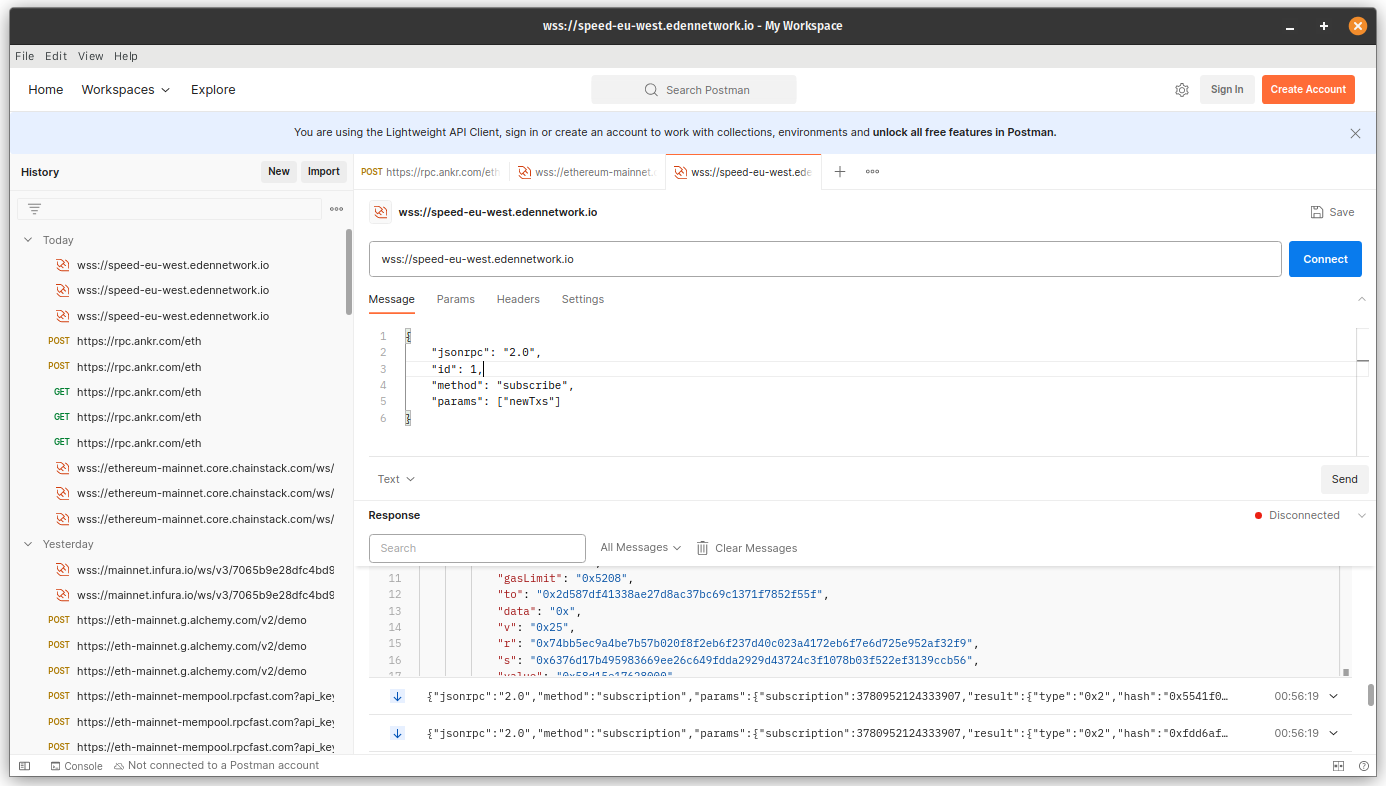
\includegraphics[width=1\linewidth]{img//screenshots/Screenshot from 2023-12-16 00-58-51.png}
\end{figure}

A continuación se deja fragmentos de la conversación con el desarrollador para futuras referencias 
\begin{verbatim}
This is the instruction on how to access the mempool streaming service: 

Alpha endpoint (speed-eu-west.edennetwork.io) is located in the EU West WebSocket url: 

wss://speed-eu-west.edennetwork.io 
wss://speed-us-east.edennetwork.io/ 
wss://speed-tokyo.edennetwork.io/ 

Pass the relevant parameter in params field. newTxs: Delivers transaction data in parsed 
format, depending on its type. See return data types below 

wscat -c wss://speed-eu-west.edennetwork.io 
{"jsonrpc": "2.0", "id": 1, "method": "subscribe", "params": ["newTxs"]} 

There’s some extra options available but not documented, if you have any questions, 
ask you can ask for more details here. UI/UX access : https://mempool.edennetwork.io/ 
Link to documentation:
https://docs.edennetwork.io/eden-mempool-streaming-service/overview/
\end{verbatim}
El día 18 de diciembre del 2023 el desarrollador contesto en discord, este cuenta que no hay una manera nativa de filtrado 
\begin{figure}
    \centering
    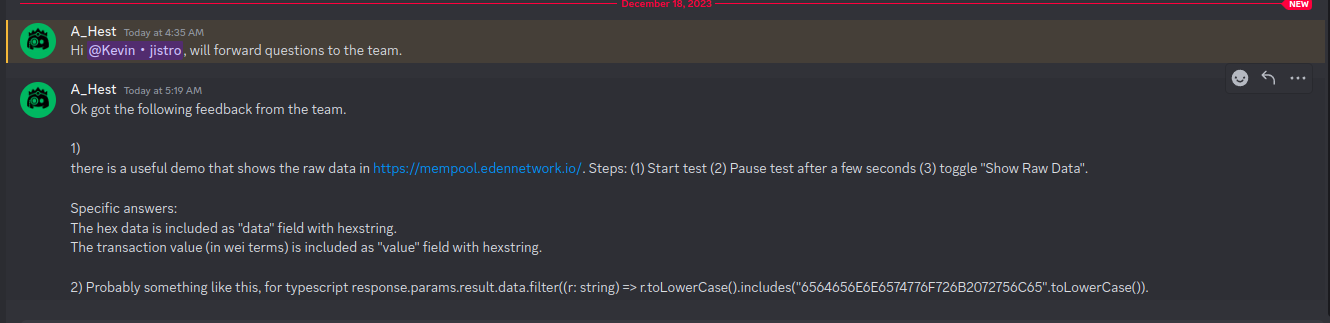
\includegraphics[width=1\linewidth]{img//screenshots/Screenshot from 2023-12-18 13-01-00.png}
\end{figure}

%---------------------------BlockNative---------------------------
\clearpage
\subsection{BlockNative}

\textbf{Red disponible:} ETH (sepolia, mainnet), Polygon

\textbf{Link:} \url{https://www.blocknative.com/}

\medskip

Nos permite ver transacciones de mempool tanto por UI
\begin{figure}
    \centering
    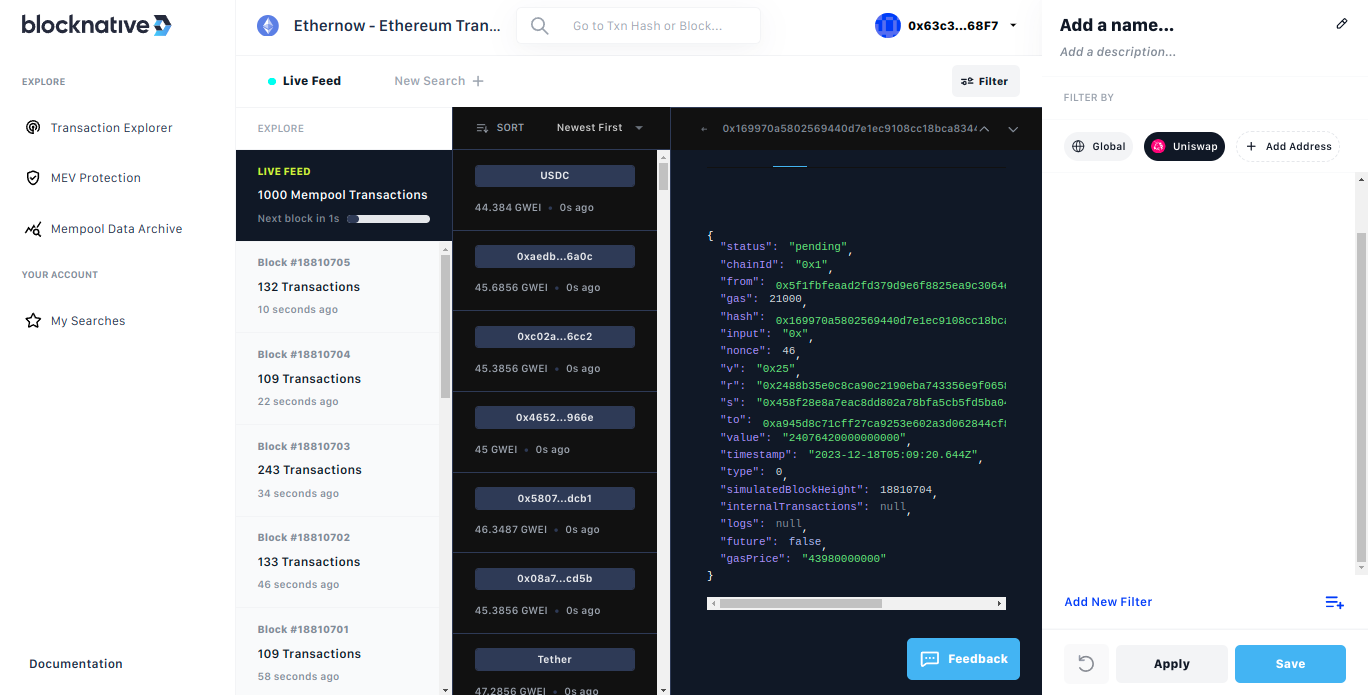
\includegraphics[width=1\linewidth]{img//screenshots/brave_screenshot_ethnopw.png}
\end{figure}

Como el la API agregando direcciones que se quieren observar (\url{https://docs.blocknative.com/mempool-tools/webhook-api#add-address-to-watch-1}) y de allí filtrar.

Sin enbargo, el filtrado es limitante permitiendo solo 
\begin{multicols}{3}
\begin{itemize}
    \item Status
    \item From
    \item To
    \item Type
    \item Value
    \item Gas
    \item Gas price
    \item Max fee per gas
    \item Max priority fee per gas
\end{itemize}
\end{multicols}

Se ha solicitado en el disord de BlockNative  el filtrado por input \url{https://discord.com/channels/542403978693050389/1019958399565303888/1186129526808395796}

El 18 de diciembre nos respondieron preguntando acerca de ese parametro que intentamos filtrar (\url{https://discord.com/channels/542403978693050389/1019958399565303888/1186509090466308188}), se ha respondido conforme lo solicitado y se espera mas respuesta de ellos.

\begin{figure}
    \centering
    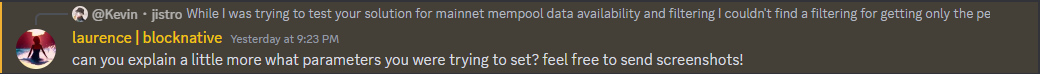
\includegraphics[width=1\linewidth]{img//screenshots/imagesc.png}
\end{figure}

%---------------------------Chainstack---------------------------
\clearpage
\subsection{Chainstack}

\textbf{Link:} \url{https://chainstack.com/}

\textbf{Redes disponibles (en EVM):} ETH (Goerli, Sepolia, Mainnet), BSC, Polygon, ARB, AVAX, BASE, OP, Scroll, Gnosis y  Starknet

\medskip

Nos permite escuchar mediante websocket las tx pendientes que se agregan a la mempool, contiene la misma data que blocknative sin filtrado \url{https://docs.chainstack.com/reference/ethereum-native-subscribe-newpendingtransactions#eth_subscribenewpendingtransactions-code-examples}

\begin{figure}
    \centering
    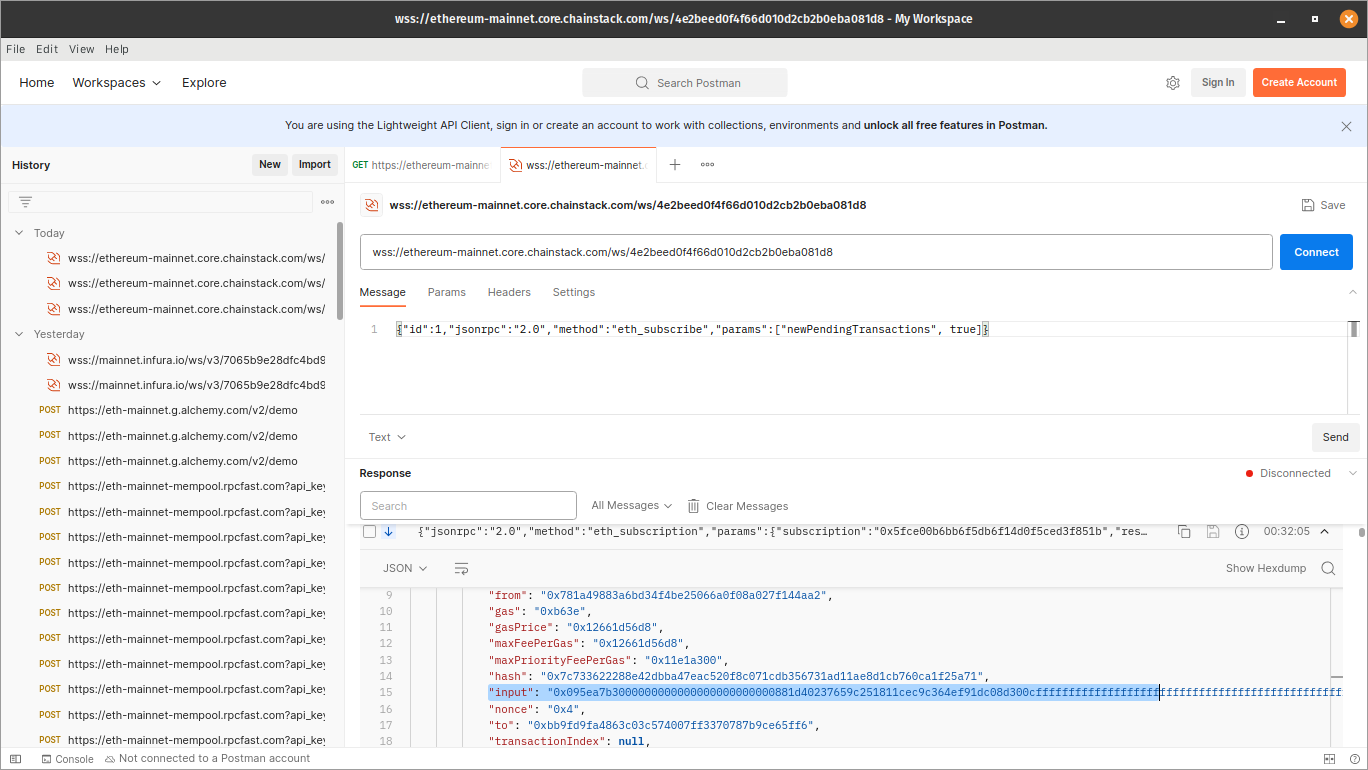
\includegraphics[width=1\linewidth]{img//screenshots/Screenshot from 2023-12-16 00-35-17.png}
\end{figure}

Se pregunto en el discord del filtrado de transacciones por lo cual ellos respondieron que hay una funcion en su API que puede ser posible de usar para nosotros \url{https://discord.com/channels/847645538093629441/989194750043250708/1186163808209739826}

\begin{figure}
    \centering
    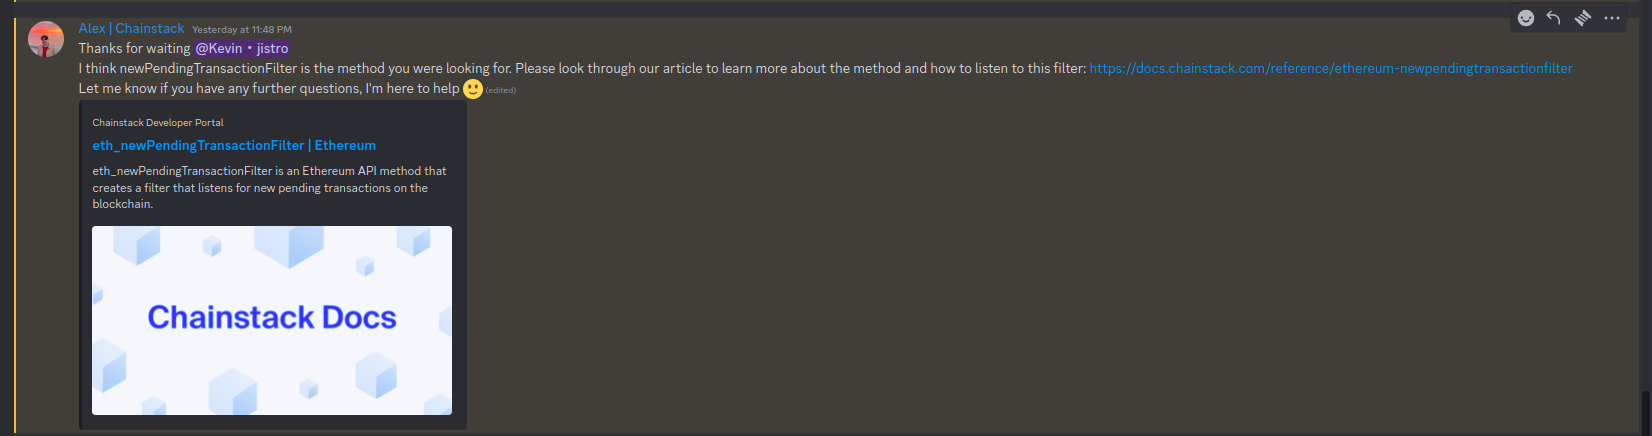
\includegraphics[width=1\linewidth]{img//screenshots/Screenshot from 2023-12-18 13-15-12.png}
\end{figure}

Uno del equipo de Chainstack me envió un mensaje promocionando sus servicios, quiero imaginar que es por el mensaje a el grupo de telegram de RPC Fast en el que preguntamos si cuentan con un streaming de mempool

\begin{figure}
    \centering
    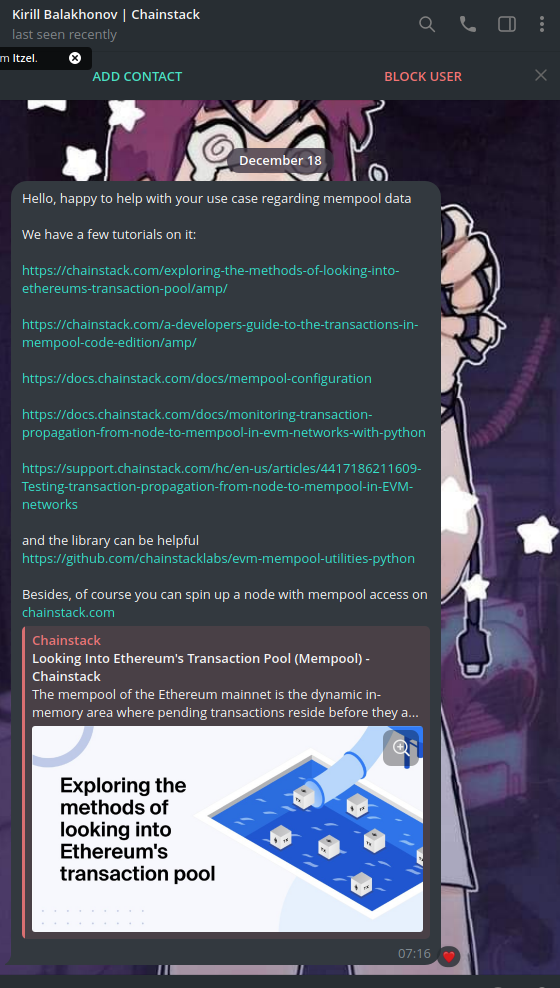
\includegraphics[width=.4\linewidth]{img//screenshots/Screenshot from 2023-12-18 12-51-25.png}
\end{figure}


Al probar dicha función sugerida antes mencionada se observo que funciona correctamente pero para ello debes generar un script donde puedas filtrar exitosamente lo que buscamos, se pregunto de nuevo en el discord si hay una manera mas directa de hacer eso. \url{https://discord.com/channels/847645538093629441/989194750043250708/1186772544586534953} 

El 20 de noviembre respondieron y lamentablemente no cuentan con ese tipo de llamadas directas y sugirieron otros métodos mediante script \url{https://discord.com/channels/847645538093629441/989194750043250708/1186840187171508315}


% ------------------------------------------------------------------------------
% NUEVA SECCIÓN
% ------------------------------------------------------------------------------
\clearpage
\section{En espera de su soporte: Mempool aparentemente limitado}
%---------------------------Streamingfast---------------------------
\subsection{Streamingfast}

\textbf{Link:} \url{https://rpcfast.com/}

\medskip

Según el FAQ de streamingfast no podemos acceder a datos de mempool

\begin{figure}
    \centering
    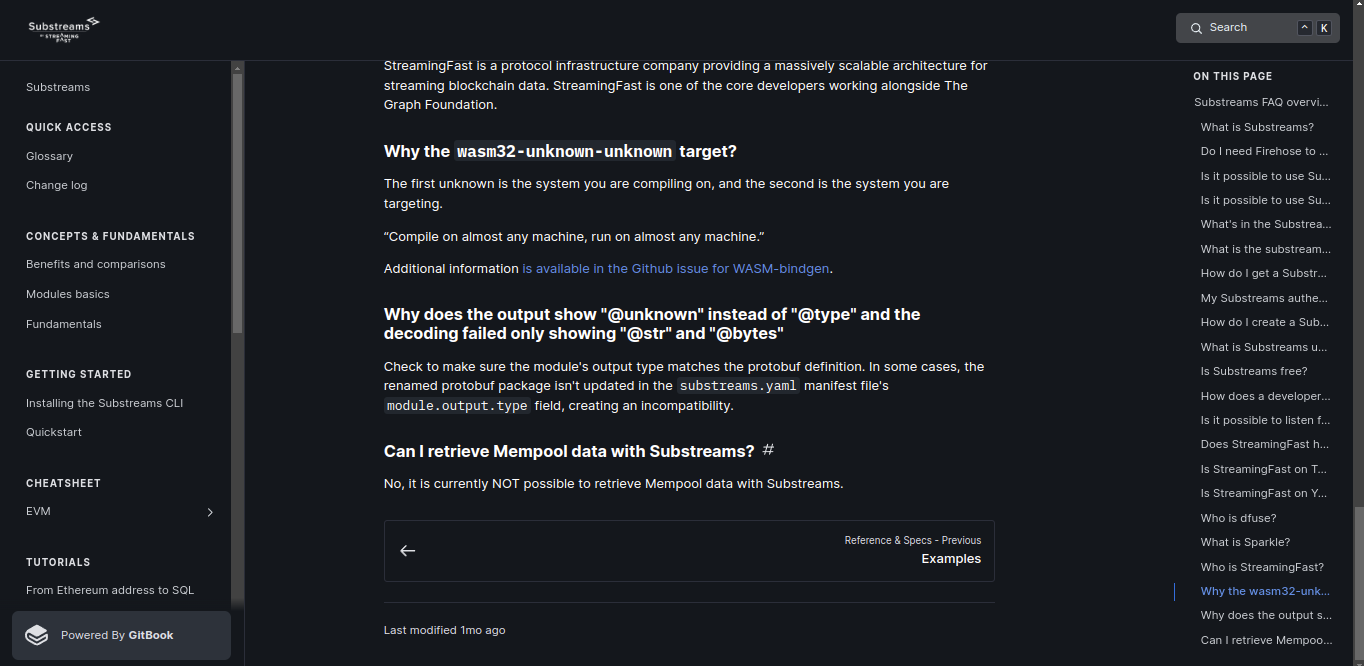
\includegraphics[width=1\linewidth]{img//screenshots/Screenshot from 2023-12-15 23-32-19.png}
\end{figure}

Nos contactamos con ellos por discord acerca de la posibilidad de que se pueda acceder a la mempool utilizando su solución 

\url{https://discord.com/channels/666749063386890256/820011680842907761/1186131875341815918}

El 18 de diciembre del 2023, crearon un hilo interno en el discord en el cual explicaron que no esta en su roadmap pero que le comentaría al equipo sobre esa posibilidad

\begin{figure}
    \centering
    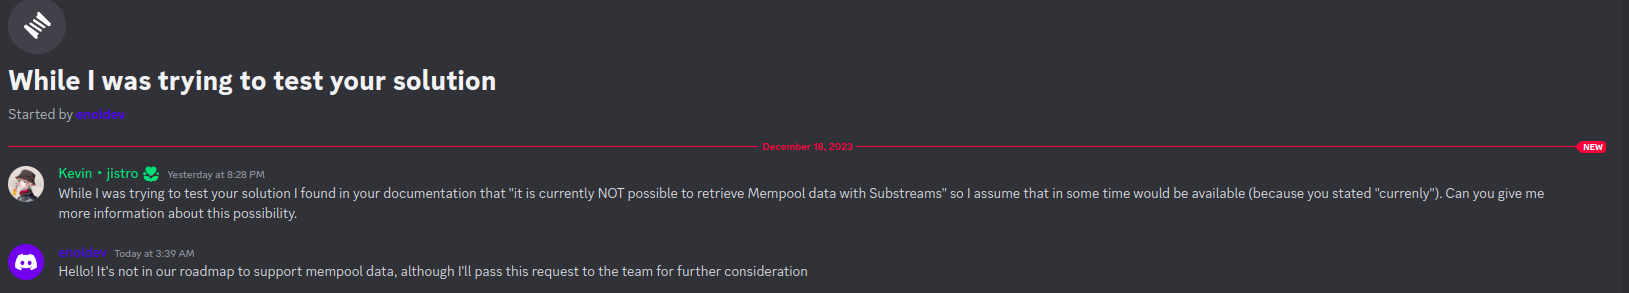
\includegraphics[width=1\linewidth]{Screenshot from 2023-12-18 13-36-09.png}
\end{figure}

\clearpage
%---------------------------Alchemy---------------------------
\subsection{Alchemy}

\textbf{Link:} \url{https://www.alchemy.com/}

\medskip

Tiene una función solo para web de mempool, sin embargo este solo puede escuchar desde el rpc server que solicitaste y no te devuelve el data

\begin{figure}
    \centering
    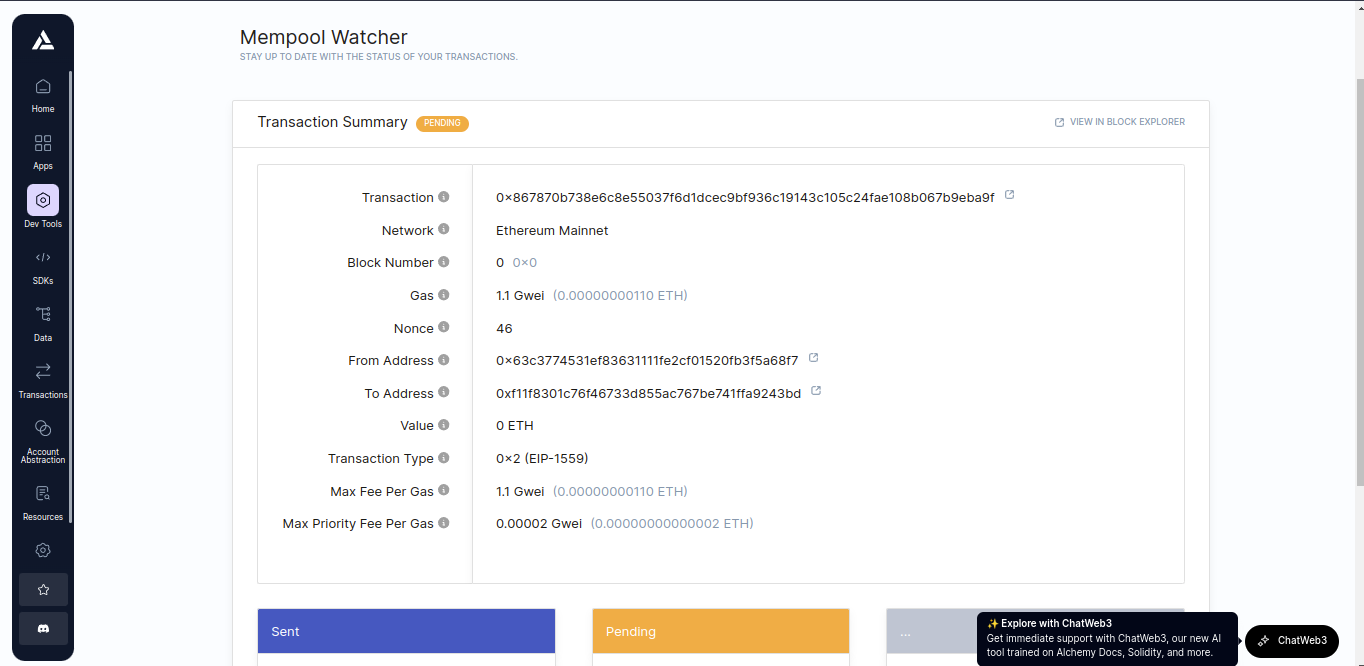
\includegraphics[width=1\linewidth]{img//screenshots/Screenshot from 2023-12-15 23-53-11.png}  
\end{figure}

Preguntamos en discord si esta función de streaming con filtros en mempool podría ser incluida en próximas actualizaciones de Alchemy \url{https://discord.com/channels/735965332958871634/736241366257893416/1186134011823783977}

El 18 de diciembre, un integrante del equipo de Alchemy creo un hilo interno en discord mostrando su interés y que vería la posibilidad de agregar esa función en Alchemy

\begin{figure}
    \centering
    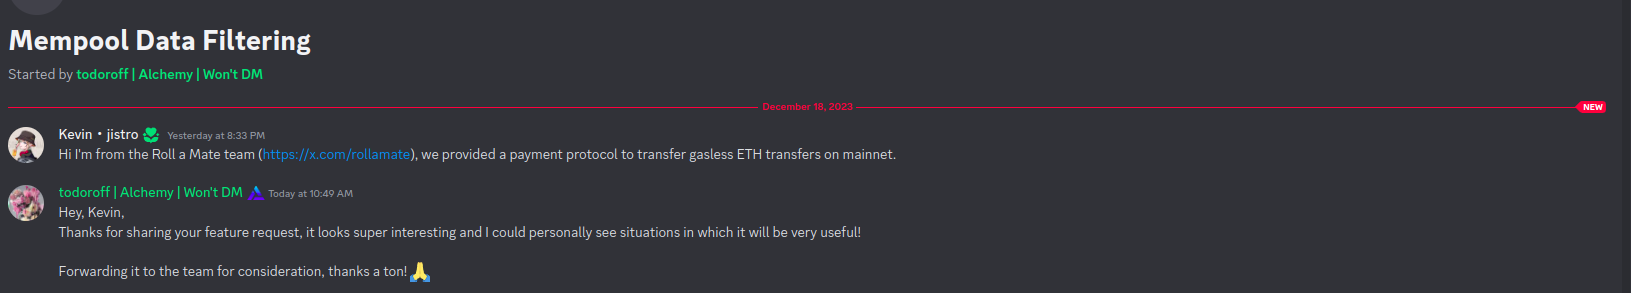
\includegraphics[width=1\linewidth]{img//screenshots/Screenshot from 2023-12-18 13-38-23.png}
    
    
\end{figure}

\clearpage
%---------------------------Etherscan---------------------------
\subsection{Etherscan}

\textbf{Link:} \url{https://etherscan.io/}

\textbf{Redes disponibles:} ETH (testnet, mainnet)

\medskip

Investigando en Etherscan se noto la presencia de un explorador de mempool \url{https://etherscan.io/txsPending}, pero en su API no muestra ninguna función para ello

\begin{figure}
    \centering
    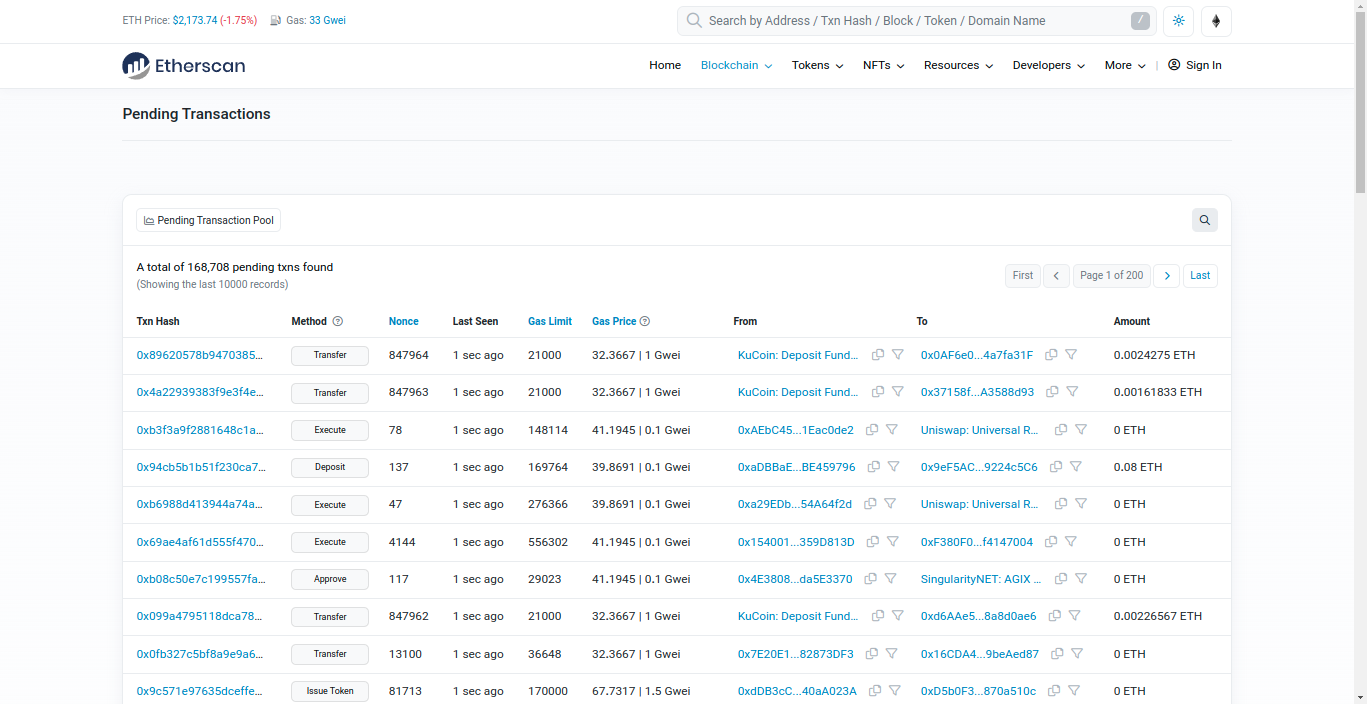
\includegraphics[width=1\linewidth]{brave_screenshot_etherscan.io.png}
\end{figure}

Se pregunto en \url{https://etherscan.io/contactus} acerca de la implementación en su api para escucha y filtrado de transacciones en mempool

\begin{figure}
    \centering
    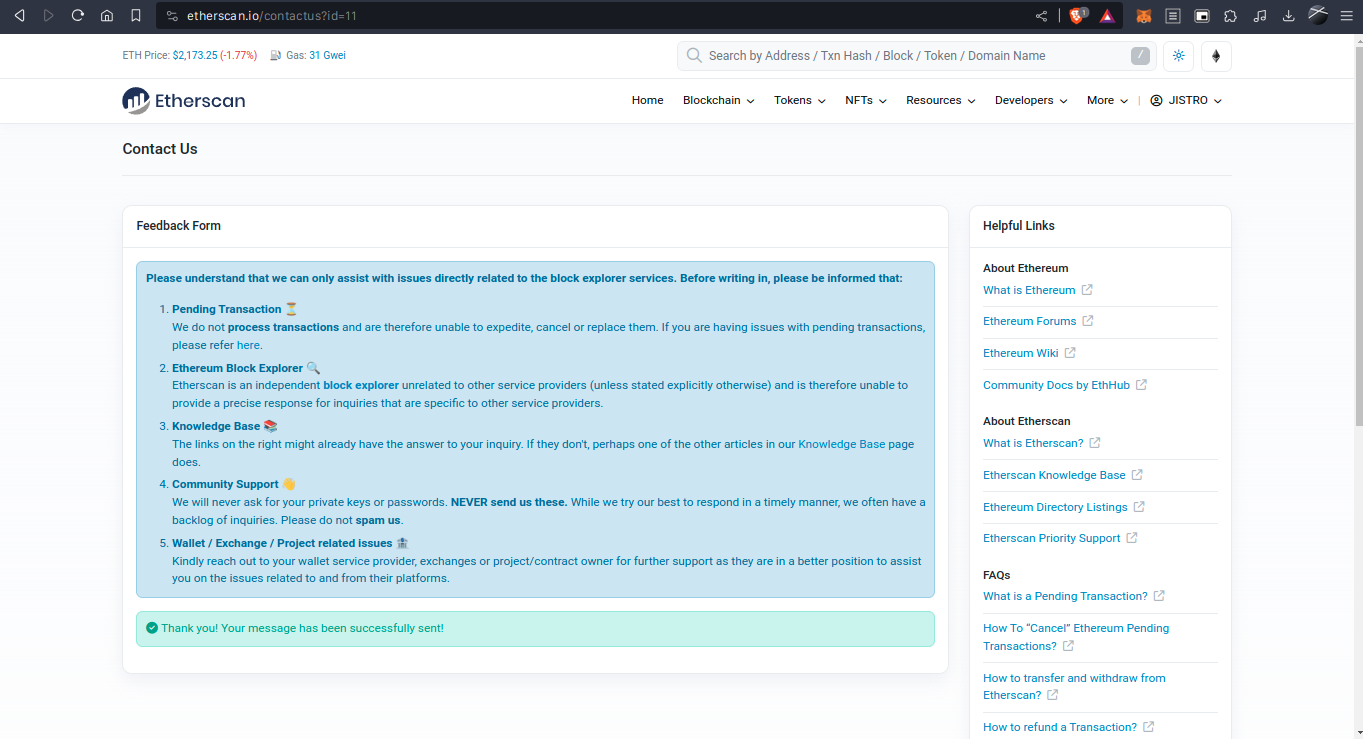
\includegraphics[width=1\linewidth]{img//screenshots/Screenshot from 2023-12-18 00-42-27.png}
\end{figure}
\clearpage
%---------------------------bloXroute---------------------------
\subsection{bloXroute}

\textbf{Link:} \url{https://bloxroute.com/}

\textbf{Redes disponibles:} ETH (Goerli, Sepolia, Mainnet), BSC y Polygon

\medskip

La función de internalTxsMempool nos permite observar transacciones en mempool pero este tipo de solicitud esta bajo paywall se intento en la versión gratuita pero muestra que no es permitido o que expiro

\begin{figure}
    \centering
    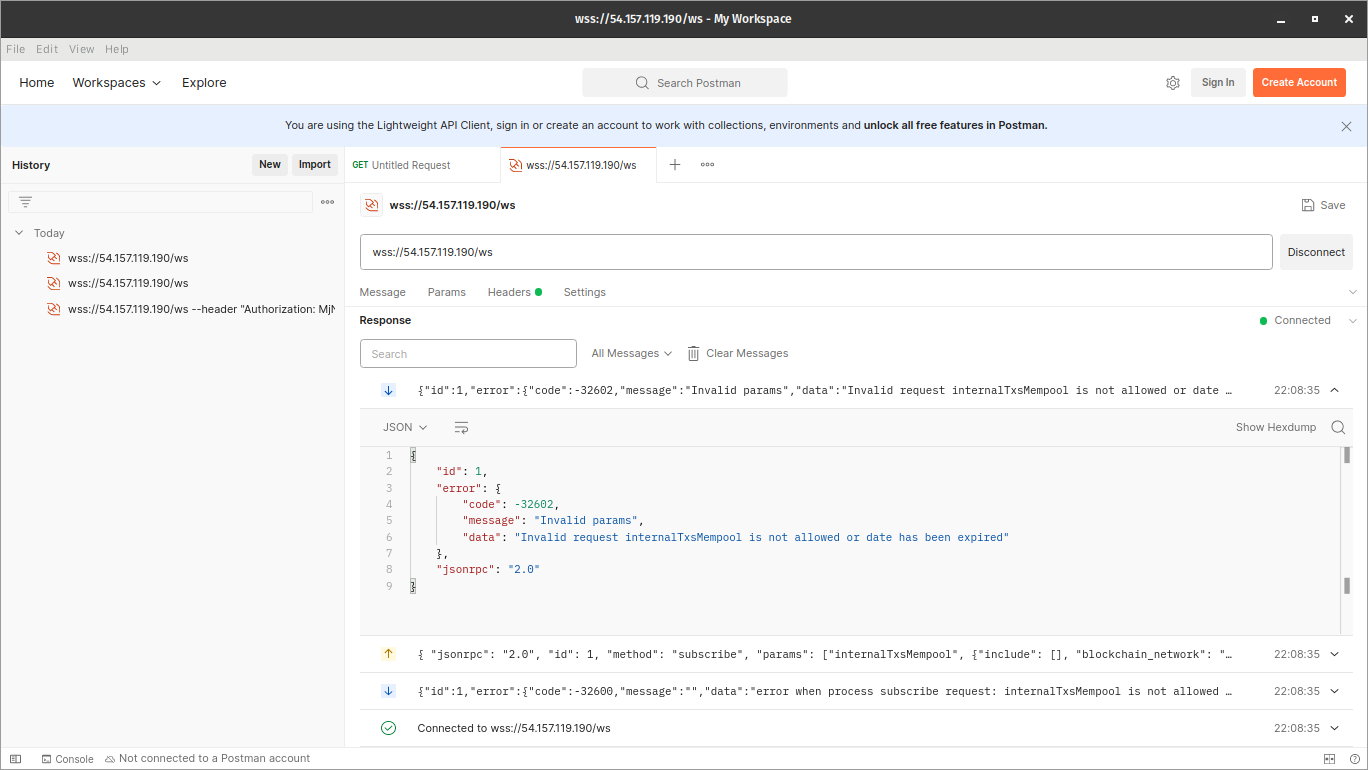
\includegraphics[width=1\linewidth]{img//screenshots/Screenshot from 2023-12-15 22-09-10.png}
\end{figure}

\url{https://docs.bloxroute.com/streams/internaltxsmempool}

no puedo deducir nada porque, aunque el ejemplo tiene demasiado detalle el paywall no me permite explorar a fondo se dejo mensaje consultando sobre la posibilidad de probarlo: \url{https://discord.com/channels/638409433860407300/638411171233398824/1186113115302146108}. Al día siguiente (18 de diciembre de 2023), respondieron que no pueden ofrecer alguna prueba del servicio \url{https://discord.com/channels/638409433860407300/638411171233398824/1186292033715970108} 

\begin{figure}
    \centering
    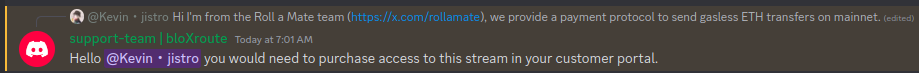
\includegraphics[width=1\linewidth]{Screenshot from 2023-12-18 13-30-41.png}   
\end{figure}
El mismo día, se pregunto si ofrecen algún tipo de demo o prueba gratuita para ver la eficacia de su servicio, el 19 de diciembre respondieron manteniendo la postura de pagar por el servicio y que el ejemplo que aparece en la decantación es suficiente como para llegar a conclusiones lo cual genera mas dudas.

\begin{figure}
    \centering
    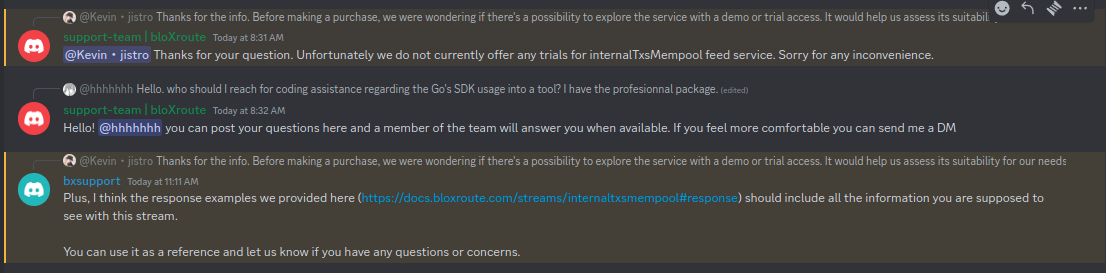
\includegraphics[width=1\linewidth]{img//screenshots/imagebXrrespuesta1901.png}
\end{figure}
\url{https://discord.com/channels/638409433860407300/638411171233398824/1186677253191503883}

Al revisar de nuevo la documentación, la sección de ''input'' se nota acotada 
\begin{figure}
    \centering
    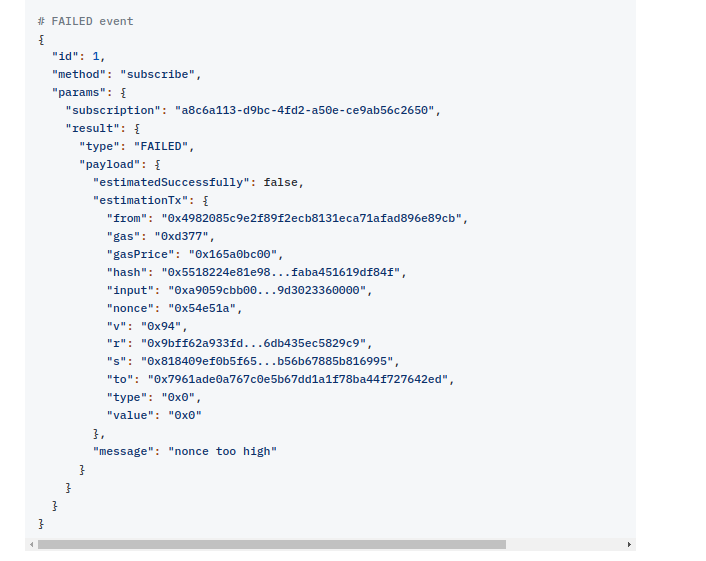
\includegraphics[width=1\linewidth]{img//screenshots/imageblox.png}
\end{figure}
Respondimos sobre esa situación, explicamos que no buscamos una prueba gratis, estamos buscando que al menos lo que se va a pagar del servicio este completo
\url{https://discord.com/channels/638409433860407300/638411171233398824/1186767623464157304}

Nos han respondido y quieren que hablemos por DM con ellos
\begin{figure}
    \centering
    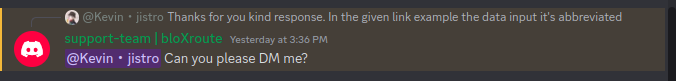
\includegraphics[width=1\linewidth]{img//screenshots/imd1122322age.png}
\end{figure}

En la conversación por DM nos mostraron un ejemplo completo de output que genera su streaming lo cual nos pareció completo sin embargo, queda la duda en que si estos datos se pueden filtrar

\begin{figure}
    \centering
    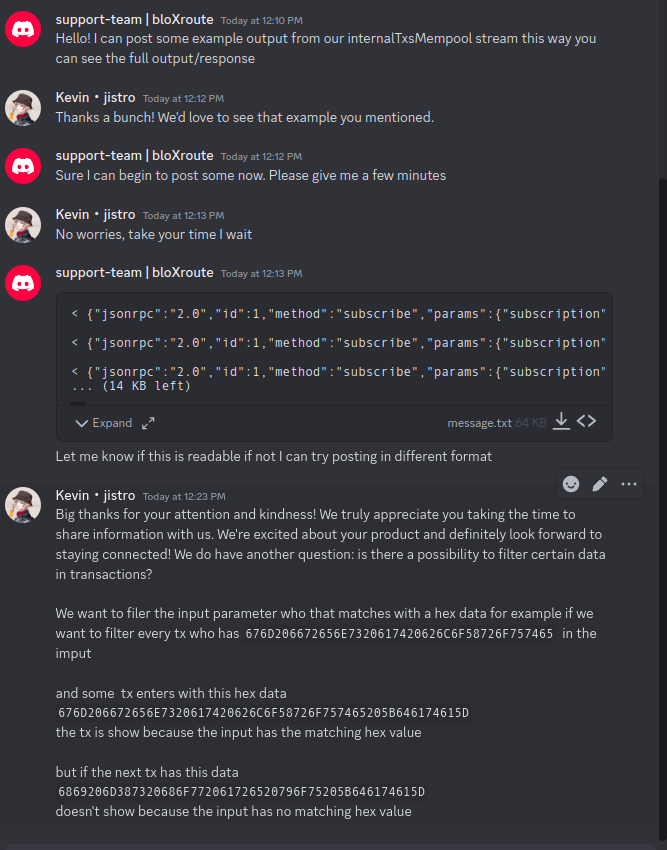
\includegraphics[width=.6\linewidth]{img//screenshots/image12321321321321.png}
\end{figure}

El 21 de diciembre el equipo de bloXroute respondió, nos indico que no hay algún método para filtrado desde la API, aun asi el stream de lo que necesitamos esta en pie 
\begin{figure}
    \centering
    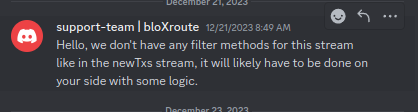
\includegraphics[width=1\linewidth]{img//screenshots/image213213123412.png}
\end{figure}


% ------------------------------------------------------------------------------
% NUEVA SECCIÓN
% ------------------------------------------------------------------------------
\clearpage
\section{No funciona: Mempool parcial o limitado}

\subsection{RPC Fast}

\textbf{Link:} \url{https://rpcfast.com/}

\textbf{Redes disponibles:} ETH (Mainnet), BSC y Polygon

\medskip

Esta permite leer transacciones en api por el hash nos devuelve los datos que nos interesan, sin embargo, parece que para obtener estos datos se necesita de un upgrade ya que al intentar usar esa instrucción de api me pide que haga ello

\url{https://docs.rpcfast.com/rpc-fast-api/ethereum-api/eth_gettransactionbyhash-ethereum}

\begin{figure}
    \centering
    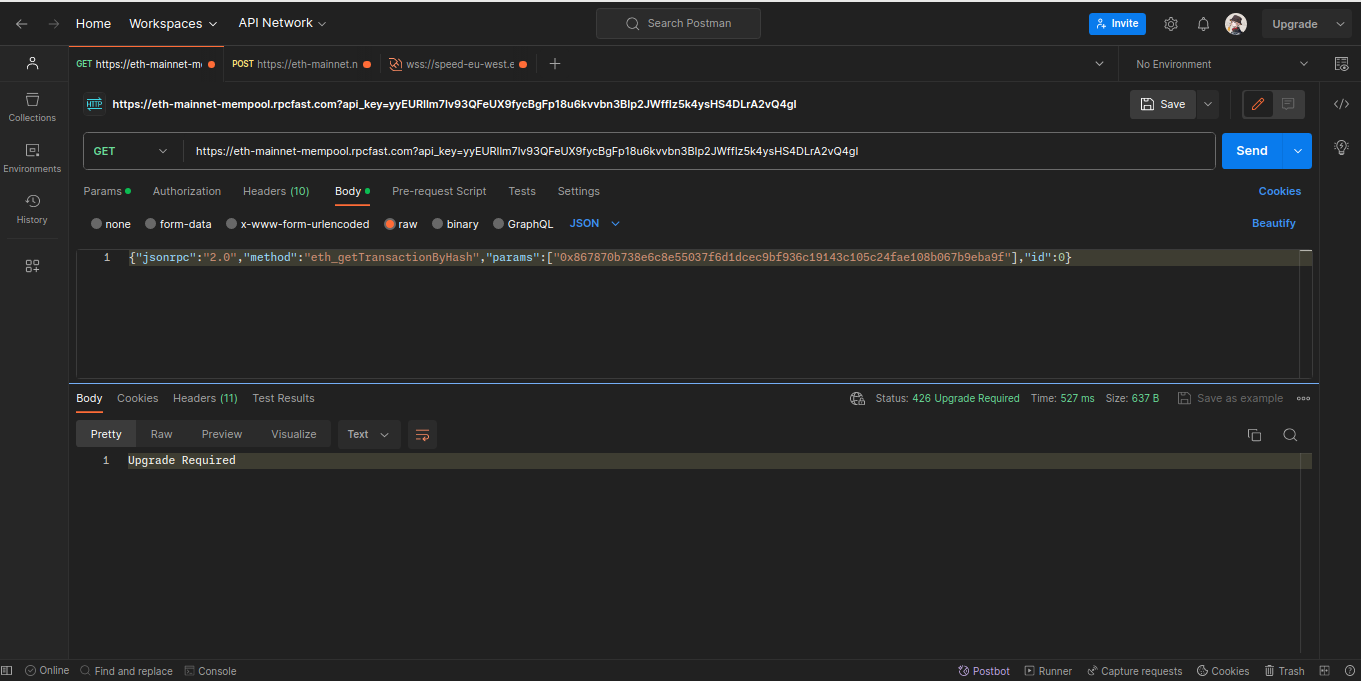
\includegraphics[width=1\linewidth]{img//screenshots/Screenshot from 2023-12-17 00-07-19.png}
\end{figure}

En el grupo de telegram \url{https://t.me/web3_infraen} se pregunto alguna alternativa o servicio para leer un streaming del mempool, el 18 de diciembre del 2023, respondieron que no cuentan con un servicio de streaming y filtrado de mempool

\begin{figure}
    \centering
    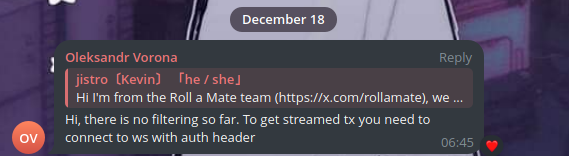
\includegraphics[width=1\linewidth]{Screenshot from 2023-12-18 13-33-23.png}
    
    
\end{figure}

\clearpage
\subsection{Infura}

\textbf{Link:} \url{https://www.infura.io/}

\medskip

Su api permite ver las transacciones pendientes y concluidas mediante el transaction hash \url{https://docs.infura.io/networks/ethereum/json-rpc-methods/eth_gettransactionbyhash}

\begin{figure}
    \centering
    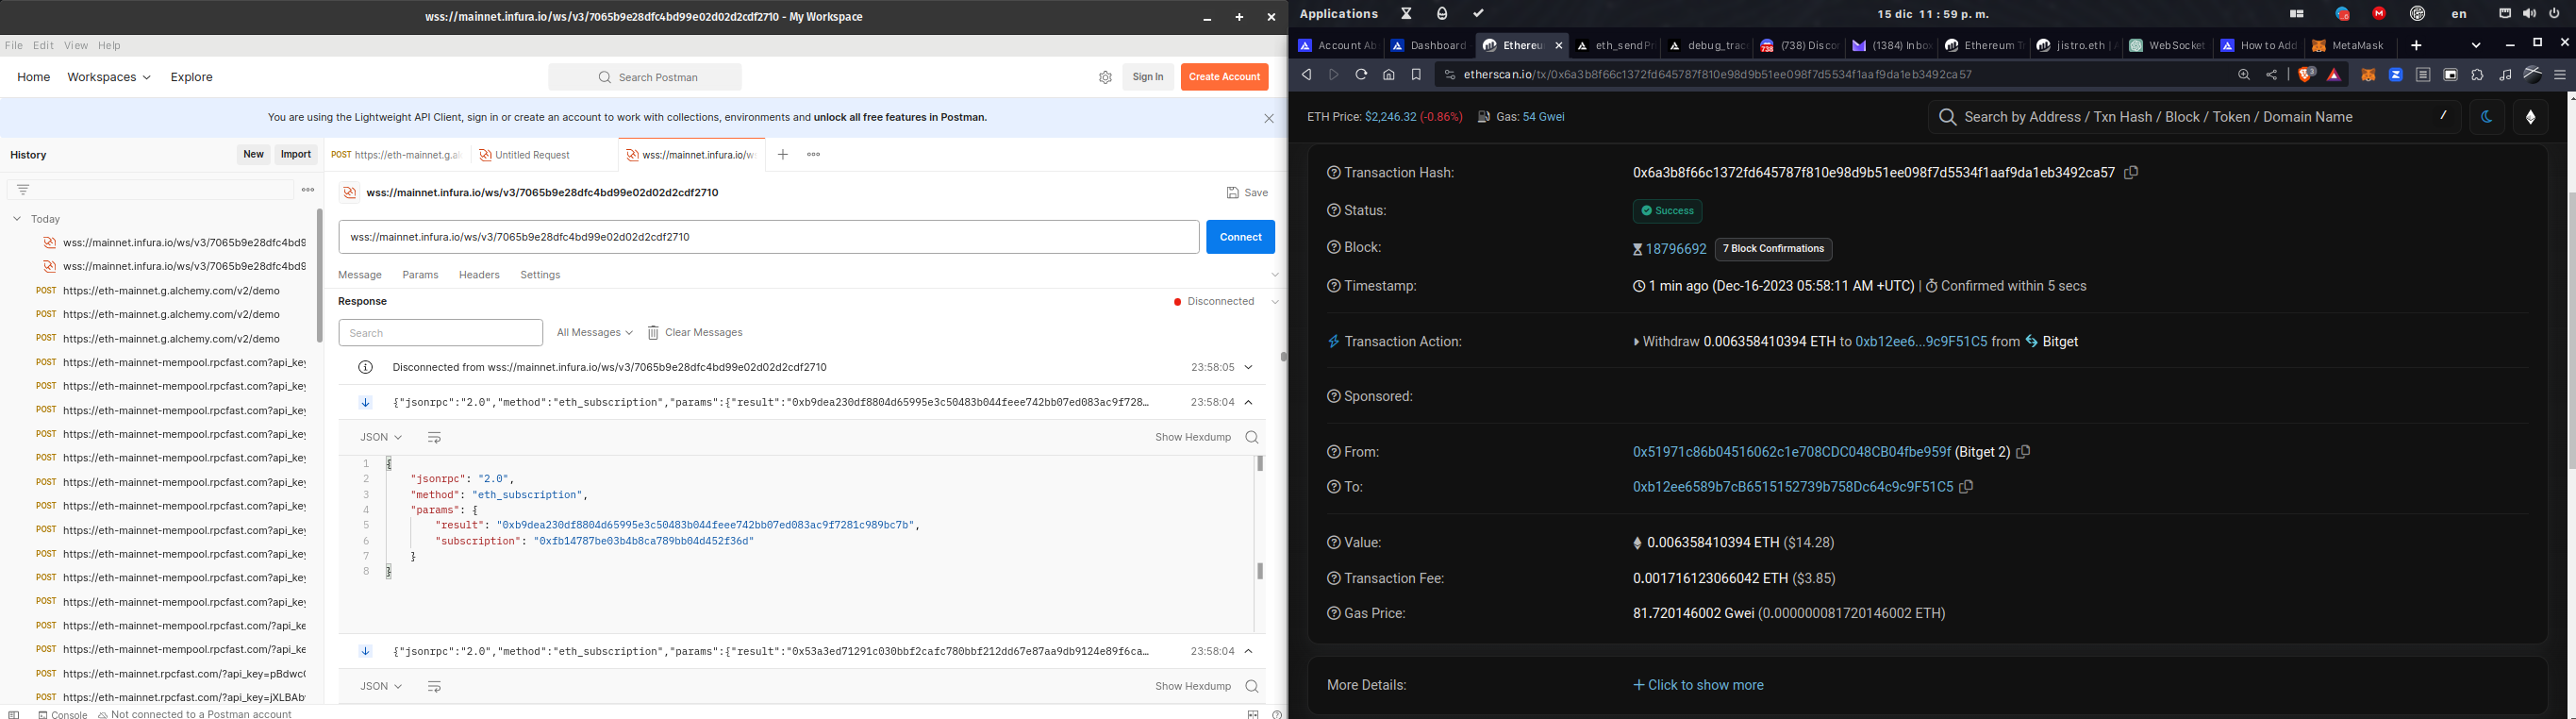
\includegraphics[width=1\linewidth]{img//screenshots/Screenshot from 2023-12-15 23-59-44.png}
\end{figure}

Se contacto en el discord de Consensys sobre la posibilidad de hacer streaming de mempool ademas de filtrado de sus datos. \url{https://discord.com/channels/697535391594446898/931191328442822666/1186136413348057158}
\clearpage
\subsection{Ankr}

\textbf{Link:} \url{https://www.ankr.com/}

\textbf{Redes disponibles (en EVM):} ETH (sepolia, mainnet), BSC, Polygon, ARB, AVAX, BASE, OP, Scroll, Gnosis y  Celo

\medskip

Con eth\_getTransactionByHash nos permite ver el hash de la transacción no importa si es en mempool o esta en el bloque, puede funcionar pero solo si conocemos el hash de la tx \url{https://www.ankr.com/docs/rpc-service/chains/chains-api/ethereum/#eth_gettransactionbyhash}

\begin{figure}
    \centering
    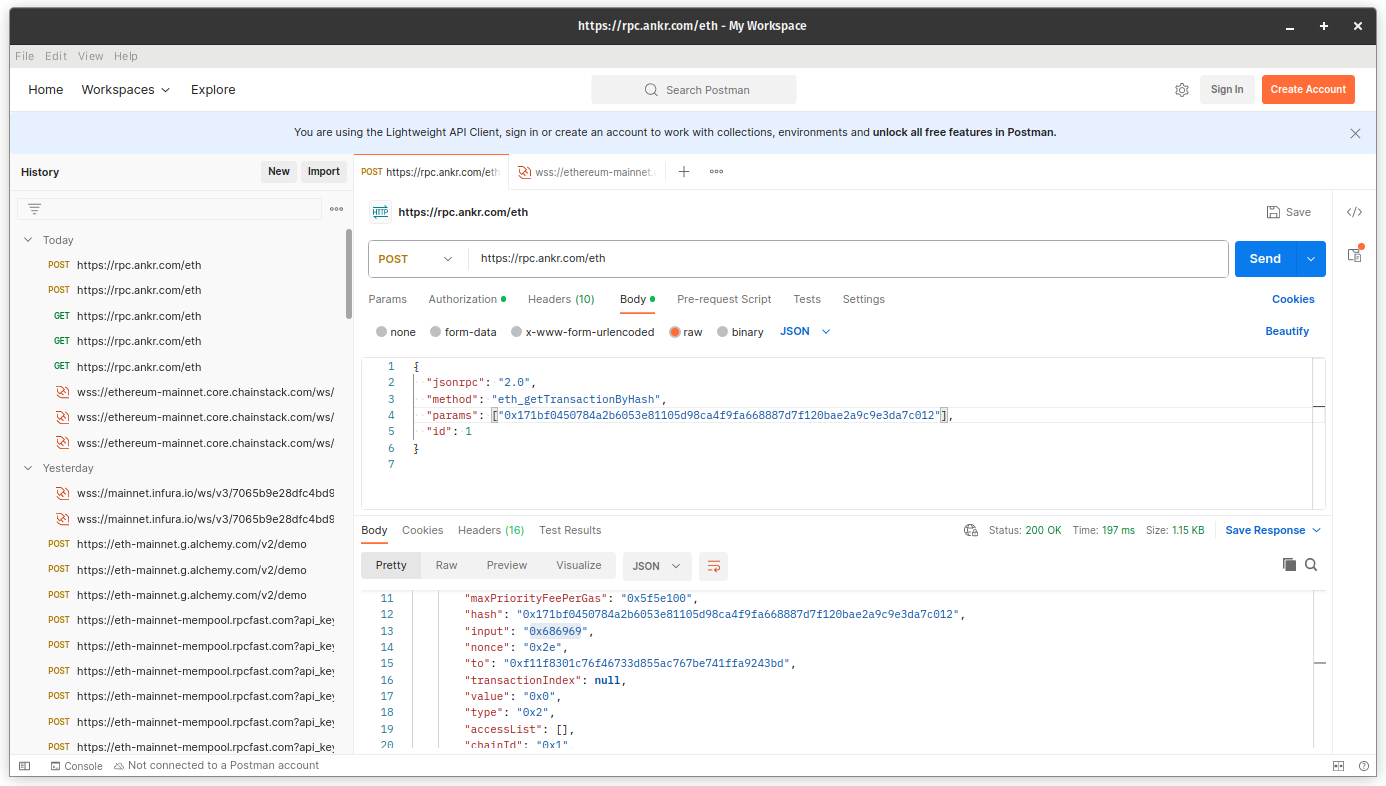
\includegraphics[width=1\linewidth]{img//screenshots/Screenshot from 2023-12-16 00-45-50.png}
\end{figure}

Se contacto por discord para solicitar el streaming y filtrado en mempool  mediante el uso de sus APIs

\url{https://discord.com/channels/795634526918279179/803991180441682030/1186147660936265850}

El 22 de Diciembre del 2023 nos respondieron que podríamos solicitar un ticket para explicar dicha situación. \url{https://discord.com/channels/795634526918279179/803991180441682030/1187824157619138570}

\begin{figure}
    \centering
    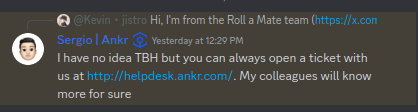
\includegraphics[width=.5\linewidth]{img//screenshots/images32432dsr34.png}
\end{figure}

Después de esto se tramito el ticket con la referencia EUS-6659 para el correo contact@jistro.xyz

\begin{figure}
    \centering
    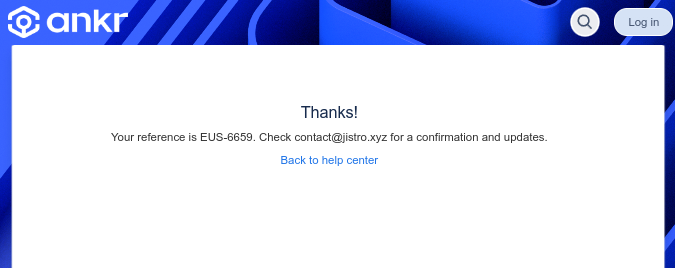
\includegraphics[width=1\linewidth]{img//screenshots/image4595841654.png}
    
    
\end{figure}
El primero de enero del 2024 nos respondieron contando que lo que sabe hasta ahora es que podemos escuchar transacciones pendientes (mempool) usando el hash de la transacción, se ha respondido el mensaje explicando que queremos un streaming y filtrado de transacciones y si hay la posibilidad de alguna demo o el poder habilitar el desarrollo para nosotros.
\begin{figure}
    \centering
    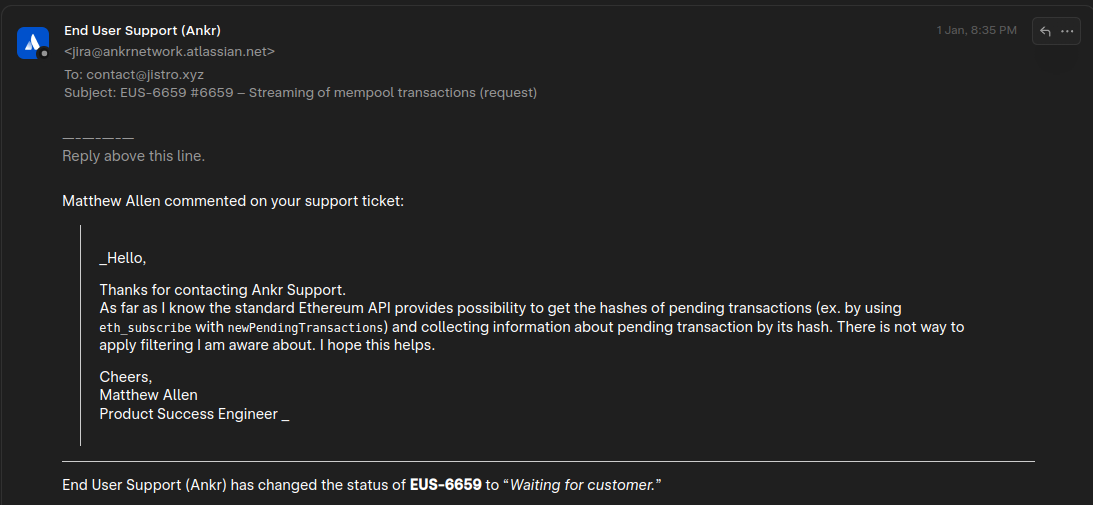
\includegraphics[width=1\linewidth]{img//screenshots/imageankr23123123.png}
\end{figure}

Hasta la fecha de edicion (13 de enero del 2014) no se ha tenido respuesta de Ankr

\clearpage
\subsection{QuickNode}

\textbf{Link} \url{https://www.quicknode.com/}

\textbf{Redes disponibles (en EVM):} ETH (Goerli, Sepolia, Mainnet), BSC, Polygon, ARB, AVAX, BASE, OP, Scroll, Gnosis y Celo

\medskip

Indagando en la documentación existen 3 maneras (que ellos) indican de como leer la mempool, una de ellas es mediante el uso de POST en su API mediante \textit{parity\_pendingTransactions} 
\url{https://www.quicknode.com/guides/ethereum-development/transactions/how-to-access-ethereum-mempool}
Esta nos devuelve datos de la mempool que han sido stremeados, pero, a diferencia de WebSockets este solo nos manda un limite de transacciones y no de manera continua 

\begin{figure}
    \centering
    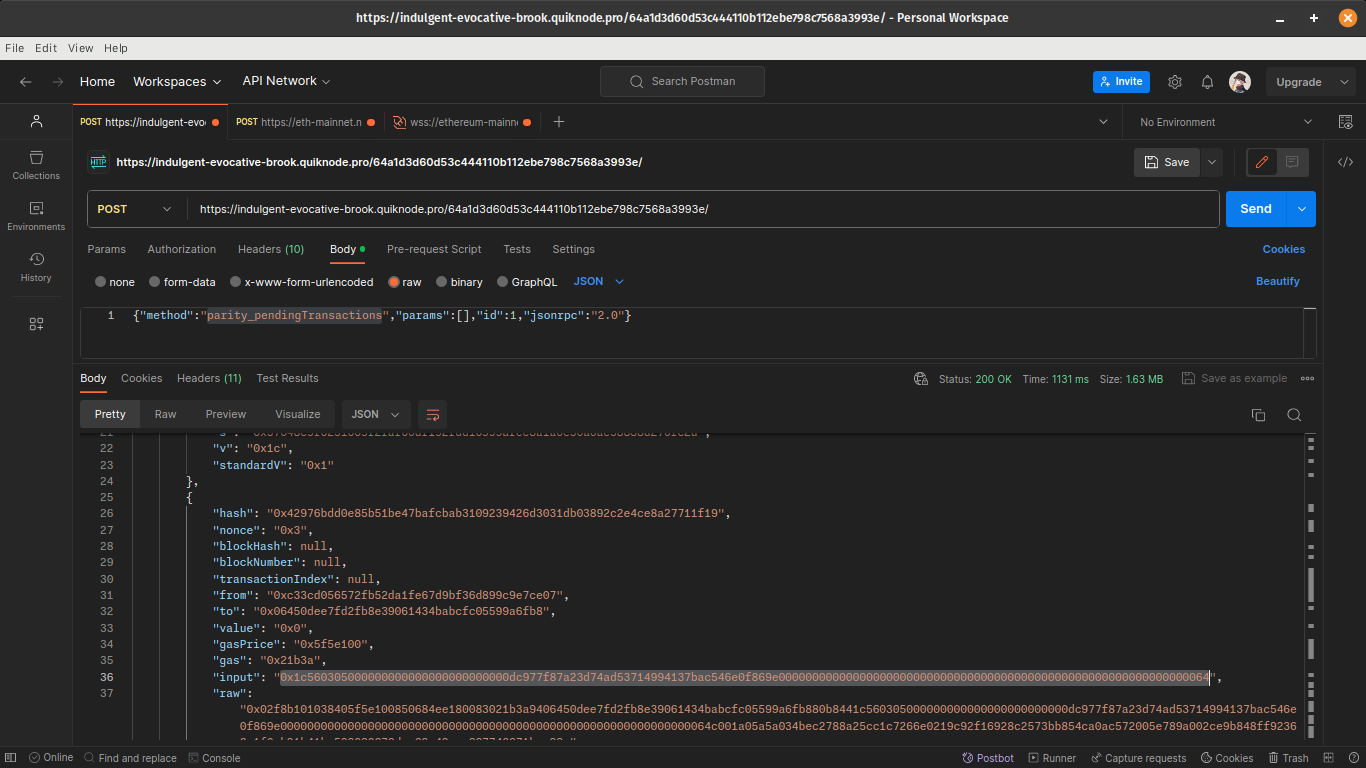
\includegraphics[width=1\linewidth]{img//screenshots/Screenshot from 2023-12-18 00-01-52.png}
\end{figure}

Investigando sobre maneras de contacto con ellos por discord se encontró con un link que lleva a una invitación no disponible y el su Luma se encontró que no cuentan con el grupo de discord, por lo que se asume que el grupo en su momento existía pero ya no se encuentra disponible

\begin{figure}
    \centering
    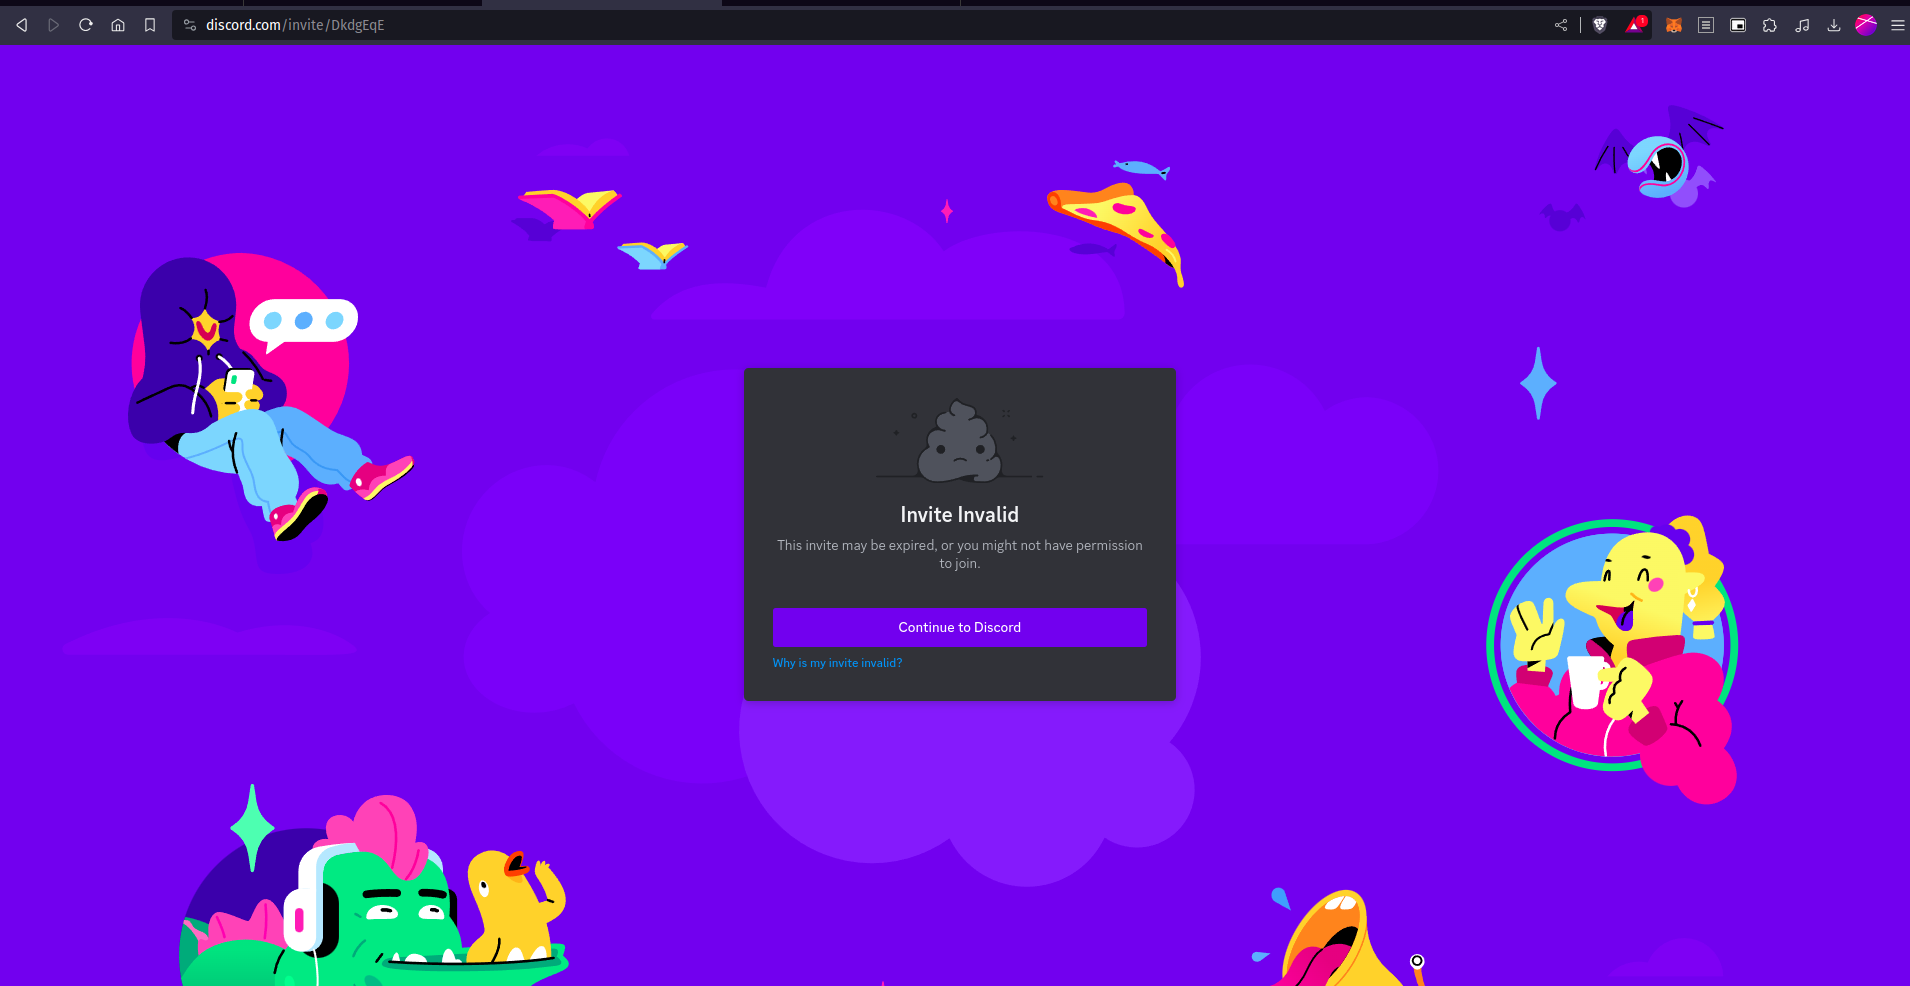
\includegraphics[width=1\linewidth]{Screenshot from 2023-12-18 15-09-14.png}
    
    
\end{figure}

\begin{figure}
    \centering
    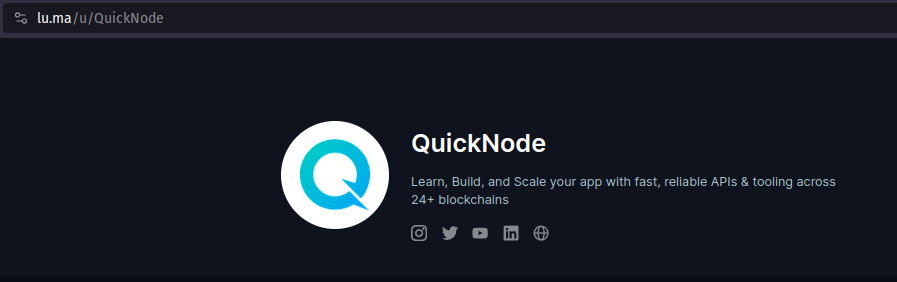
\includegraphics[width=1\linewidth]{img//screenshots/Screenshot from 2023-12-18 15-09-37.png}
    
    
\end{figure}
